\documentclass[12pt,onecolumn,twoside]{article}
\usepackage[T1]{fontenc}
\usepackage[utf8]{inputenc}
\usepackage{amsfonts, amsmath}
% \usepackage{nature}

\usepackage{cell}
\usepackage{natbib}
% The Cell style only works with BibTeX and not BibLaTeX. So load the 'cell' package here, the bib and style file commands in the document at the end, and make sure the cell.bst file is in the same directory as the tex file. Once all of this is in place, compile on the terminal with this sequence: xelatex filename, bibtex filename.aux, xelatex filename, xelatex filename. Atom-latex is a bit unreliable in this regard.

\usepackage[document]{ragged2e} %For non-justified text alignment
\usepackage[margin=0.75in]{geometry}
\usepackage{fontspec}
\setmainfont{Carlito}
\usepackage{hyperref}
\hypersetup{
	colorlinks = true, %Colours links instead of ugly boxes
	urlcolor = blue, %Colour for external hyperlinks
	linkcolor = red, %Colour of internal links
	citecolor = black %Colour of citations
}
%\usepackage{threeparttable}
\usepackage{graphicx}
\usepackage{caption}
\usepackage{subcaption}
% \usepackage{fancyhdr}
% \pagestyle{fancy}
% \fancyhf{}
% \rhead{\thepage}
\makeindex

\usepackage{authblk}
\author{Vibishan B.}
\affil{Department of Biology, Indian Institute of Science Education and Research (IISER), Pune}

\title{Experimental evolution under a dual selection regime of dispersal and chronic larval malnutrition in \textit{Drosophila melanogaster}}
\date{\empty}

\begin{document}
	\maketitle
	\section{Introduction}

	% \subsection{Dispersal}
	Dispersal is defined as the movement of individuals or propagules across with potential consequences for gene flow \citep{Ronce2007}, and as such, is a key component of life history strategy \citep{Clobert2012, Bonte2017}. It is a multi-stage process that includes departure, inter-patch movement and settlement, and is an important part of an organism's response to changing environmental conditions. However, dispersal is also a highly energy-intensive process that could incur many kinds of costs across its various stages \citep{Bonte2012}. These could be due to direct energetic allocation to the movement process (rover vs sitter morphs in Drosophila larvae \cite{Vijendravarma2012}), developmental processes for sensory apparatus involved in condition-dependent dispersal behaviour, or even behavioural changes that could improve chances of settlement success. Such energetic requirements make a compelling case for the development of trade-offs between dispersal and other aspects of an organism's life history.

	Previous work from our lab has investigated the evolution of dispersal using an experimental evolution approach by which fruit fly populations were selected for ambulatory dispersal over long distances for several generations. Interestingly, it was found that although multiple components of dispersal did respond to the selection \citep{Tung2018}, no costs were observed in body weight, fecundity or lifespan while the metabolomic profiles showed a clear shift to an energy-deprived state in the selected flies compared to control flies \citep{Tung2018a}. The apparent lack of costs to dispersal evolution is surprising, and suggests that the banana-jaggery medium on which the flies are maintained was rich enough in energy for the selected flies to allocate to dispersal without having to suffer costs for other traits. We therefore adopt a similar experimental evolution approach to study the evolution of dispersal under more nutrient-poor conditions. We subject the flies to larval malnutrition by raising the eggs in a modified banana-jaggery medium with one-third the normal concentration of dry yeast, which is the primary source of protein in the medium. In the sequence of our protocol, eclosed adults are subjected to dispersal selection on the 12th day post-egg collection. These ``malnourished dispersers" are therefore under a dual selection regime, in which they must complete development in a protein-deficient food source and also complete dispersal over a certain path length as adults in order to reproduce. Their physiological state would therefore be strongly affected by larval nutrition, since compensatory feeding at the adult stage is not allowed at the point of dispersal.
	% \begin{itemize}
	% 	\item Dispersal is recognised as an important partner in life history evolution.
	% 	\item Dispersal is costly, and is correlated to several phenotypes, physiological and behavioural. Dispersal syndromes are defined through patterns of covariation between morphological, physiological and behavioural traits \cite{Clobert2012}.
	% 	\item Previous work from the lab has shown that under normal lab conditions, at least components of dispersal can be evolved without any significant cost across many traits (except for dessication and some infections) considered key in life history strategies.
	% 	\item Could it be that the nutritional content of the maintenance food is such that all flies have enough excess energy to allocate for dispersal alongside everything else?
	% 	\item Whole-food dilution is somewhat hairy, and early trials showed that N/3 had the same effect as diluting all components.
	% \end{itemize}

	% \subsection{Larval malnutrition}

	\paragraph{\empty} In the dual selection regime described above, the larval malnutrition treatment alone, apart from dispersal selection, also allows for a parallel exploration of selective outcomes along the nutrition axis by comparing the non-dispersing control populations from the malnutrition regime with the ancestor populations maintained on normal food from which they were derived.

	Evolutionary responses to dietary modifications are well-documented in the literature. Poor larval diet affects body size and foraging \citep{Ahmad2018, Vijendravarma2012}, and could improve egg-to-adult viability and developmental time even though the plastic response to changes in diet remained unaffected \citep{Kolss2009}. The physiological consequences of single-generation diet changes are even more widely known to affect lifespan, fecundity and body size, apart from many other traits \citep{Lee2008, Tatar2014, Musselman2011, Skorupa2008}. There is some evidence to argue that the single-generation effects of dietary changes are not driven by the exact calorific content of the food \citep{Mair2005}, and instead that the ratio of certain macronutrients in the food might play a stronger role in larval and adult physiology \citep{Tatar2014, Lihoreau2016}; the picture is far from clear. We therefore employ four isocaloric diet treatments with different proportions of protein and carbohydrates to address a two-part question: (a) does selection under larval malnutrition change the plastic response of fruit flies to dietary changes in protein:carbohydrate ratio? (b) is the plastic response driven by the calorific content of the food, or a particular balance of macronutrients? While the effects of nutrition-based selection and dietary modifications have been explored independent of each other, our plan brings together these distinct lines of investigation by asking if selection history affects the reaction norm of responses to dietary modification.
	% \begin{itemize}
	% 	\item Our paradigm involves malnutrition at the larval stages => larvae grow in one-third the regular amount of protein.
	% 	\item With or without compensatory feeding, this marks an imbalance in the regular diet of the larvae.
	% 	\item Imbalanced diets have physiological consequences, as shown by the long and storied history of dietary restriction and nutritional geometry in flies.
	% 	\item With these physiological effects as a starting point, it is possible to ask if these proximate mechanisms change reaction norms over the course of adaptation to an imbalanced diet.
	% \end{itemize}
	% \citep{Ahmad2018}-body size is affected by levels of dietary protein and sugars, foraging stuff from below, and cannibalism. PI3K/Akt has potential connections to many of these processes.
	% \citep{Vijendravarma2012}-sitter-rover type polymorphism seen between selected and control populations, under abundant low-quality food. Increase in foraging rate (longer foraging paths, etc) is energy-intensive, and could therefore depend on amount and quality of food. Under crowded conditions, increasing foraging length could lead to better food patches, while uncrowded poor-food environments can possibly not sustain a high-foraging phenotype due to poor food quality. They see their selected populations acting as sitters compared to the unselected ones, and while \textit{for} expression does not follow this expectation, other genetic mechanisms involving \textit{for} are possible.
	% \citep{Kolss2009}-evolutionary response to poor food included better egg-to-adult viability, smaller body size and faster development time in poor food, but the plastic response to food quality was mostly the same as the unselected flies. Selected female flies had lower fecundity on normal food compared to unselected ones, but no other trade-offs were found in heat or cold tolerance. Adult survival on normal food is not different between the two, while adults from selected larvae survived worse on poor food; in both these cases, larvae were raised on normal food.
	\section{Methods}
	\subsection{Experimental evolution protocol}
	We begin with four independent large outbred populations (breeding population size \textasciitilde 2400) of \textit{Drosophila melanogaster} ($\text{VBC}_{\text{1-4}}$, short for ``Vagabond Control") in the lab which in turn were derived from similar older lines (${\text{DB}}_{\text{1-4}}$: ``Dey Baseline"). From each $\text{VBC}_{i}$, two populations called ${\text{MD}}_{i}$ (“Malnourished Dispersers”, selected for dispersal under malnourished conditions) and ${\text{MC}}_{i}$ (corresponding control for only dispersal) were derived. All populations with the same subscript constitute one block, and populations with the same subscript are related by ancestry. All MD(C) populations are maintained on a 15-day cycle at 25$^{\circ}$C and constant light conditions. For each population, eggs from each new generation are reared on malnourished (N/3 Y) food. On day 12 post egg collection, eclosed adult MD flies were introduced into a migration apparatus for dispersal selection (Figure \ref{fig0}). Briefly, the set-up consists of three components: source, path and destination. For every generation of ${\text{MC}}_{i}$, adult flies are introduced into a source container without food or water on the 12th day post-egg collection, and allowed to disperse (currently, a path length of 15m) for 6 hours or till \textasciitilde 50\% of the flies reach the sink, whichever occurs first. MC populations, at the same time, are kept in source containers under identical conditions for the same duration without undertaking migration.
	\begin{figure}
		\centering
		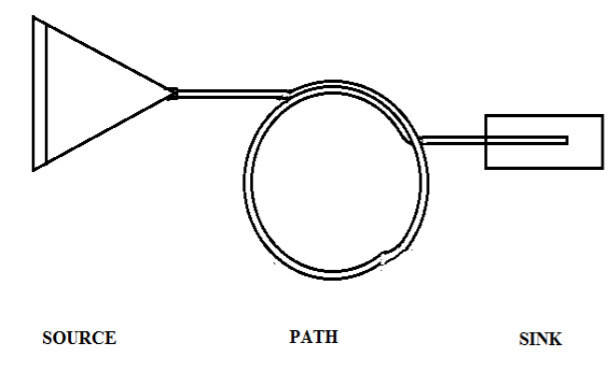
\includegraphics[width=0.5\textwidth, keepaspectratio]{path.png}
		\caption{\label{fig0} Migration setup used for dispersal selection}
	\end{figure}
	\subsection{Dispersal evolution}
	Following 42-43 generations of selection according to the protocol above, assays were carried to determine if any adaptive response has developed in MD compared to MC in response to the dispersal selection regime. All experiments were performed two blocks at a time due to logistic constraints, and after one generation of relaxation to eliminate maternal effects.
	\subsubsection{Dispersal kernel}
	The dispersal kernel is a probability-density function, usually of the distances travelled by a population of dispersers in a given period of time \citep{Clobert2012}. The kernel is a central feature of any dispersal process and can be useful to measure as it carries information about propensity to initiate dispersal, the spatial extent of the population, and potential for change in the distribution.
	The assay setup is similar to the migration apparatus shown in Figure \ref{fig0}, with a path length of 20m. The path is made up of detachable sections of plastic pipes, referred to as bins (twenty 0.5m + ten 1m bins). 12 days post egg collection, ~1000 flies per treatment were introduced into a source (as in Figure 1)  and allowed to disperse for six hours. After six hours, the bins were sequentially detached and sealed. The flies were heat-killed and the number of male and female flies in each bin were counted. For each MD(C) population, 3 replicates were run in parallel two blocks at a time, resulting in a total of \textasciitilde 12,000 flies used for the kernel experiment.

	Two separate components were calculated based on the resulting kernel:
	\[
		\text{Propensity} = \frac{\text{\# of flies outside the source}}{\text{Total \# of flies}}
	\]
	\[
		\text{Ability} = \sum_{i=1}^{y} \frac{x_{i}n_{i}}{n_{i}}
	\]

	where, $y$ is the total number of bins, $n_{i}$ is the number of flies in the $i^{th}$ bin, and $x_{i}$ is the distance of the mind-point of the $i^{th}$ bin from the source.

	In effect, propensity measures the proportion of flies in the source container that initiated dispersal and ability measures the average distance travelled over the flies that did leave the source container.

	\subsubsection{Dry body weight}
	12 days post egg collection, flies were sorted by sex under light CO$_\text{2}$ anaesthesia, then placed in 1.5mL Eppendorf tubes (20 individuals per tube; 10 replicates per treatment for each sex), and killed by flash freezing. These flies were dried in the tubes at 60$^{\circ}$C for 72h and the weight of each Eppendorf tube was measured to the closest 0.1mg on a digital weighing balance, first with and then without the flies. The average body weight per fly was calculated as: $\frac{\text{Weight of the Eppendorf tubes with flies - Weight of empty tubes}}{\text{\# of flies in the tube}}$.
	\subsubsection{Fecundity}
	This assay was conducted 14 days post egg collection in which 55 male-female pairs per treatment were each kept in a 50mL Falcon tube (with holes for aeration). The lid contained a small food cup providing a flat surface for oviposition. These set-ups were left undisturbed for 12 hours in a well-lit environment maintained at 25°C. After 12 hrs, the flies were discarded and the number of eggs laid on the food was counted under a microscope.
	\subsubsection{{Locomotor activity (DAM)}}
	Locomotor activity and resting behavior of adult male flies was assayed using the Drosophila Activity Monitoring (DAM2) data collection system (Trikinetics Inc, Waltham, MA) following standard protocols (\cite{Chiu2010}; see also Text S1.2.1 therein). 12 days post egg collection, individual flies were introduced into small glass tubes (length 6.5 cm, diameter 5 mm; 32 replicates per treatment). These tubes were placed in the monitoring apparatus such that two independent perpendicular IR beams pass through the centre of each glass tube. The activity was recorded for 6 h. The activity for a given fly was estimated as the average number of times the fly crossed the IR beam per hour \citep{Chadov2015}. Continuous inactivity for five minutes or more was considered as sleep/rest \citep{Hendricks2000, Chiu2010}.

	\subsection{Dietary modification}
	We used the MC and VBC populations for these experiments which were performed over all four blocks.

	All assays were conducted after rearing both MC and VBC on normal food for one generation to minimise any potential non-genetic parental effects. This was done two blocks at a time for logistic reasons. A cornmeal formulation was used for the experimental diets as it allows finer control of protein:carbohydrate ratios in the food through yeast and sucrose-yeast acted as the protein source while sucrose acted as the carbohydrate source. Eggs collected from the relaxed populations were reared on cornmeal medium of four different protein:carbohydrate (P:C) concentrations-lowY, eqY, highY and onlyY, corresponding to final w/w ratios of yeast to sucrose of 1:3, 1:1, 3:1 and 1:0 respectively. The amounts of all other components (cornmeal, water and agar) were the same between the four diets. Adults eclosing subsequently were assayed for key life-history traits as below.
	\subsubsection{Egg-to-adult viability}
	Exactly 30 eggs were collected per vial for 10 vials per treatment. The number of flies eclosed was counted under $\text{CO}_{2}$ anaesthesia daily from the 8th day post egg collection till the 14th day.
	\subsubsection{Dry body weight}
	12 days post egg collection, flies were sorted by sex under CO2 anaesthesia, then placed in 1.5mL Eppendorf tubes (8-12 individuals per tube; 10 replicates per treatment for each sex), and killed by flash freezing. These flies were dried in the tubes at 60$^{\circ}$C for 72h and the weight of each Eppendorf tube was measured to the closest 0.001mg on a digital weighing balance, first with and then without the flies. The average body weight per fly was calculated as: $\frac{\text{Weight of the Eppendorf tubes with flies - Weight of empty tubes}}{\text{\# of flies in the tube}}$.
	\subsubsection{Realised fecundity}
	14 days post egg collection, \textasciitilde 40 male-female pairs per treatment were kept in a vial with 6mL normal banana jaggery food and left to lay eggs for 12h in a well-lit environment maintained at 25$^{\circ}$C. After 12h, the flies were discarded and the vials were maintained under similar conditions. The number of flies eclosed per day was counted every day from the 8th day post egg collection till the 14th day under CO$_\text{2}$ anaesthesia.

	\subsection{Statistical analyses}
	Multi-way mixed-model ANOVAs were used wherever applicable. All ratio data were arcsine-square root transformed and block was considered a random factor wherever it occured in the analysis. All analyses were performed on R, using functions from the \texttt{lmerTest} package for fitting mixed-effects models and generating ANOVA tables.

	\section{Results and discussion}
	\subsection{Dispersal evolution}
	Figures \ref{fig1} and \ref{fig2} summarise the findings on the evolution of dispersal traits in our fly populations. Both properties of the dispersal kernel measured here show a significant response to the selection regime. For all assays, multi-factor mixed-effects ANOVAs were used, with population (and sex, in Figure \ref{fig1}) was considered a fixed factor and block was modelled as a random effect.
	MD have higher propensity ($F_{(1, 5)}$ = 49.4, $p$ = 0.0007) as well as ability ($F_{(1, 3)}$ = 42.071, $p$ = 0.0074) than MC, which means that a larger fraction of the MD population at the source initiate dispersal and on average, travel longer distances than the MC flies. It could also be inferred from these two observations that MD have a larger spatial extent than MC and a more even distribution over the dispersal path. This would lead to a flatter kernel curve for MD than MC, since most of the latter are concentrated around the source and the first few bins.

	The kernel differences are mirrored in locomotor activity data, in which the MD flies were more active (Figure \ref{fig2c}; $F_{(1, 3)}$ = 17.37, $p$ = 0.025) and rested less than MC (Figure \ref{fig2d}; $F_{(1, 3)}$ = 13.48, $p$ = 0.035). These two quantities are mathematically independent, and therefore reflect an MD phenotype in response to the dispersal selection regime.

	\paragraph{\empty}On the other hand, dry body weight showed no response to the selection pressure, and within the two blocks tested so far, neither does fecundity. This suggests that the selection regime has worked in so far as producing an adaptive response in locomotor activity and dispersal traits, but this adaptive change does not seem to have come at the cost of either body weight or fecundity.
	\begin{figure}
		\centering
		\begin{subfigure}{0.7\textwidth}
			\scalebox{0.5}{\input{fig1a.pdf_tex}}
			\subcaption{\empty}
		\end{subfigure}
		\begin{subfigure}{0.7\textwidth}
			\scalebox{0.5}{\input{fig1b.pdf_tex}}
			\subcaption{\empty}
		\end{subfigure}
		\caption{\label{fig1} Evolution of the dispersal kernel. (a) Propensity was significantly different between the populations ($F_{(1, 5)}$ = 49.4, $p$ = 0.0007), but the sex main effect was insignificant. Propensity values were arcsine-square root transformed before analysis. (b) Ability was significantly differ between the two populations ($F_{(1, 3)}$ = 42.071, $p$ = 0.0074), but not between the sexes. All plots are mean $\pm$ SD. }
	\end{figure}
	\begin{figure}
		\centering
		\begin{subfigure}{0.49\textwidth}
			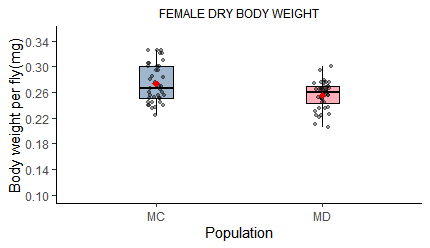
\includegraphics[width=\textwidth, keepaspectratio]{fig1c.png}
			\subcaption{\label{fig2a}\empty}
		\end{subfigure}
		\begin{subfigure}{0.49\textwidth}
			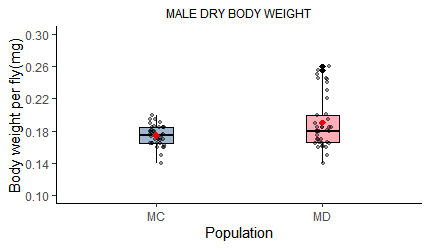
\includegraphics[width=\textwidth, keepaspectratio]{fig1d.png}
			\subcaption{\label{fig2b}\empty}
		\end{subfigure}\\
		\begin{subfigure}{0.49\textwidth}
			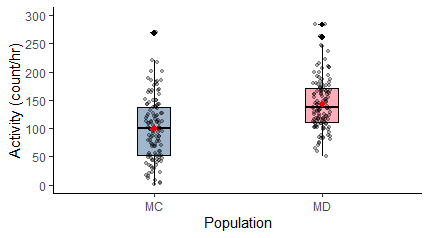
\includegraphics[width=\textwidth, keepaspectratio]{fig1e.png}
			\subcaption{\label{fig2c}\empty}
		\end{subfigure}
		\begin{subfigure}{0.49\textwidth}
			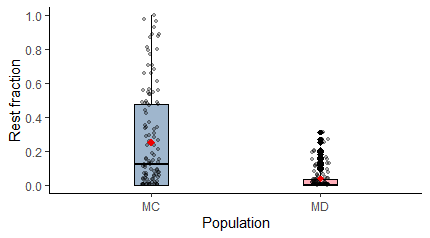
\includegraphics[width=\textwidth, keepaspectratio]{fig1f.png}
			\subcaption{\label{fig2d}\empty}
		\end{subfigure}
		\begin{subfigure}{0.49\textwidth}
			\centering
			\scalebox{0.6}{\input{fig2.pdf_tex}}
			\subcaption{\label{fig2e}\empty}
		\end{subfigure}
		\caption{\label{fig2} Trait correlations with evolving the dispersal kernel. Body weight is not significantly different between the two populations in (a) females or (b) males; (c) Average activity count per hour was significantly higher in MD than in MC ($F_{(1, 3)}$ = 17.37, $p$ = 0.025), while (d) fraction of rest bouts was significantly lower in MD ($F_{(1, 3)}$ = 13.48, $p$ = 0.035). Rest fractions were arcsine-square root-transformed for the analysis; (e) Difference in fecundity (means $\pm$ SD are plotted here) between the two populations is unclear as the two blocks for which data are available do not show the same trends. Formal statistical analysis is awaiting data from the remaining two blocks. All boxes are IQRs, solid black lines are medians, solid red circles are means and whiskers are 1.5*IQR.}
	\end{figure}
	\begin{figure}
		\centering
		\scalebox{0.7}{\input{fig3.pdf_tex}}
		\caption{\label{fig3} Response in body weight to dietary P:C ratios; the populations did not differ from each other although there was a significant main effect on female body weight of diet ($F_{(1, 3)}$ = 24.23, $p$ = 0.00012). All plots are mean $\pm$ SD.}
	\end{figure}
	\begin{figure}
		\centering
		\begin{subfigure}{\textwidth}
			\scalebox{0.35}{\input{fig4a.pdf_tex}}
			\subcaption{\empty}
		\end{subfigure}
		\begin{subfigure}{\textwidth}
			\scalebox{0.35}{\input{fig4b.pdf_tex}}
			\subcaption{\empty}
		\end{subfigure}
		\caption{\label{fig4} Response in (a) realised fecundity and (b) egg-to-adult survivourship to dietary P:C ratios; the two populations did not differ significantly in either of the traits, but the diet main effect was significant in realised fecundity alone ($F_{(1, 3)}$ = 55.34; $p$ = 8.42*10$^{\text{-6}}$). All plots are mean $\pm$ SD.}
	\end{figure}

	\subsection{Dietary modification}

	In the MC-VBC comparison, we find that broadly, the selection pressure due to larval malnutrition in MC does not lead to different responses to dietary changes in protein:carbohydrate ratios.
	We only show the analysis for female body weight since male deaths in two of the diet treatments gave rise to highly unbalanced data for male body weight. For female body weight, the diet main effect alone was significant across both populations ($F_{(1, 3)}$ = 24.23, $p$ = 0.00012) in a 3-way mixed-effects ANOVA with population and diet as fixed factors and block as a random factor. Realised fecundity showed a similar trend, where the main effet of diet alone was significant but MC were not different from VBC ($F_{(1, 3)}$ = 55.34, $p$ = 8.42*10$^{\text{-6}}$). The trend with diet for both these traits are largely in line with published literature on the effects of diet modification \citep{Lee2008}. Egg-to-adult survivourship was affected by neither the diet nor the selection history, and was generally above 80\% across all treatments.

	\section{Future outlook}
	For dispersal evolution, the results so far raise several more questions. We find that there is a detectable response to the selection regime in at least two components of the dispersel kernel-MD show higher propensity and ability than MC. This is reflected in the locomotor activity profiles, where MD show higher activity and lower rest fraction than the MC. On the other hand, these changes appear to have taken place without a corresponding response in body weight, and to the extent tested, in fecundity.

	\paragraph{\empty}To complete this part of the picture then, completion of the fecundity dataset is therefore an immediate priority, while the response in locomotor activity in particular strongly suggests that related behavioural traits like exploration and male-male aggression might have co-evolved with dispersal. Moreover, considering the diet aspect of the dual selection regime, behavioural responses to selection might also include feeding \citep{Carvalho2005} and foraging \citep{Ribeiro2010}. Therefore, a wider description of aspects of behaviour related to malnutrition and dispersal is of importance.

	In this context, we plan to characterise exploratory behaviour and male-male aggression, protocols for which have already been standardised in the lab. Measuring food intake in Drosophila has been attempted by several methods, each with advantages and shortcomings \citep{Carvalho2005, Ribeiro2010, Shell2018, Wong2009}. We plan to use a dye uptake assay in solid food using the FD\&C blue dye, which has been shown to provide reliable estimates of amount of food consumed within a span of about 30 minutes \citep{Shell2018}.

	At the same time, it is curious that body weight still seems unresponsive to selection for dispersal despite the supposedly nutrient-poor larval environment. However, selection for dispersal could impose additional selection for the maintenance of some minimum body weight. This would obviously reduce any difference in body weight between MD and MC, but might lead MD to respond differently from MC in a situation that demands additional allocation of resources from body weight. Starvation and dessication resistance are prime candidates to follow this possibility since both are dependent on biomass, and we plan to test both.

	Whether fecundity would reveal an effect is uncertain. It has been observed in flies that protein and carbohydrates can be used distinctly for building biomass and making eggs respectively \cite{Ahmad2018, Mirth2019}. If so, the current malnutrition regime is only deficient in protein and would have sufficient carbohydrates for egg production. More detailed metabolic characterisation would then be required to determine how, if any, the cost of dispersal is manifested in MD.

	\paragraph{\empty} Concerning the diet treatments, the response in realised fecundity alone is in line with published literature (higher protein leads to higher fecundity). We set out asking two questions. The first was if selection history changes the plastic response to dietary modification. Our data so far suggests that it does not, since MC and VBC do not differ substantially in their responses in terms of body weight, realised fecundity or egg-to-adult survivourship. This lack of difference may be trivially attributed to insufficient selection pressure on MC, and we therefore require further characterisation of the MC phenotype to determine if any adaptive change has taken place in MC at all. The planned set of assays detailed above for the MD-MC comparison should provide this informatioThis change in calorific content could be achieved either by adjusting the sucrose or yeast concentration in the medium. Together, the calorific content and the particular macronutrient used to arrive at the target calorific level give rise to a factorial design that can be used for a complete exploration of landscape of dietary responses in our fly populations.

	The second question was if the response to dietary modification is calorie- or macronutrient-driven, and since we do find a response in all three traits to the dietary modification itself, this question remains active. The treatments used here were all isocaloric, and the next step is then to constitute similar diets with cornmeal medium over a range of lesser or higher calorific content.
	\bibliographystyle{cell}
	\bibliography{review}
	% \printbibliography

\end{document}
